%==============================================================================
% Sjabloon onderzoeksvoorstel bachproef
%==============================================================================
% Gebaseerd op document class `hogent-article'
% zie <https://github.com/HoGentTIN/latex-hogent-article>

% Voor een voorstel in het Engels: voeg de documentclass-optie [english] toe.
% Let op: kan enkel na toestemming van de bachelorproefcoördinator!
\documentclass{hogent-article}

% Invoegen bibliografiebestand
\addbibresource{voorstel.bib}

% Informatie over de opleiding, het vak en soort opdracht
\studyprogramme{Professionele bachelor toegepaste informatica}
\course{Bachelorproef}
\assignmenttype{Onderzoeksvoorstel}
% Voor een voorstel in het Engels, haal de volgende 3 regels uit commentaar
% \studyprogramme{Bachelor of applied information technology}
% \course{Bachelor thesis}
% \assignmenttype{Research proposal}

\academicyear{2022-2023}

\title{De kennis van de Info Support medewerkers opfrissen door het Info Support Guidance Framework te gamificeren met een quiz generator: een proof-of-concept}

\author{Manu Vleurick}
\email{manu.vleurick@student.hogent.be}

\author{Rayme Emin}
\email{rayme.emin@student.hogent.be}

\supervisor[Co-promotor]{Yoeri Van Damme (Info Support)}

\specialisation{AI \& Data Engineering}
\keywords{NLP, Question Generation, Gamificatie, Guidance Framework}

\begin{document}
    
\begin{abstract}
In dit onderzoek wordt een proof of concept in de vorm van een quiz generator gemaakt voor het Info Support Guidance Framework om te onderzoeken of dit effectief kan zijn in het opfrissen van het Guidance Framework. Het Guidance Framework is een framework waarin alle kennis die Info Support heeft opgedaan in zijn hele loopbaan staat beschreven. De quiz generator zou de medewerkers in staat kunnen stellen om op een laagdrempelige manier bij te blijven met de kennis beschreven in het framework. Een proof of concept van de quiz generator van de software oplossing wordt beschreven, waarbij flexibiliteit, gebruiksvriendelijkheid en uitbreidbaarheid van belang zijn. Er worden meerdere soorten vragen gegenereerd zoals meerkeuzevragen, waar/onwaar-vragen, invulvragen en combinatievragen. Voor elke soort vraag wordt er getest of dit relevant is tegenover de brontekst door middel van de BLUE score en manuele score-toereiking van een medewerker die het Guidance Framework gebruikt. Ook wordt er nagedacht over andere gamificatie methodes die er kunnen gebruikt worden om het Guidance Framework op te frissen.

% Hier schrijf je de samenvatting van je voorstel, als een doorlopende tekst van een paragraaf. Let op: dit is geen inleiding, maar een samenvattende tekst van heel je voorstel met inleiding (voorstelling, kaderen thema), probleemstelling en centrale onderzoeksvraag, onderzoeksdoelstelling (wat zie je als het concrete resultaat van je bachelorproef?), voorgestelde methodologie, verwachte resultaten en meerwaarde van dit onderzoek (wat heeft de doelgroep aan het resultaat?).
\end{abstract}
    
\tableofcontents
    
% De hoofdtekst van het voorstel zit in een apart bestand, zodat het makkelijk
% kan opgenomen worden in de bijlagen van de bachelorproef zelf.
%---------- Inleiding ---------------------------------------------------------

\section{Introductie}%
\label{sec:introductie}

Quizzen worden gemaakt om kennis op te frissen dat je hebt geleerd. Maar wat als die kennis blijft uitbreiden en je niet zomaar altijd een nieuwe quiz kan maken? Dit is het probleem bij het Info Support Guidance Framework. Dit is een framework waar alle kennis die Info Support heeft verzameld tijdens hun carrière in de IT consultancy wereld wordt bijgehouden. Info Support wil door middel van gamificatie technieken de kennis van hun medewerkers opfrissen. Dit gebeurt door een Proof of Concept (PoC) van een automatische quiz generator die met Natural Language Processing (NLP) technieken verschillende soorten vragen kan genereren over de onderwerpen beschreven in het Guidance Framework. De Poc zal relevante vragen moeten kunnen stellen om de essentie van de onderwerpen in het framework te toetsen. Er kunnen ook extra gamificatie technieken worden gebruikt naast de quiz.


%Waarover zal je bachelorproef gaan? Introduceer het thema en zorg dat volgende zaken zeker duidelijk aanwezig zijn:

% \begin{itemize}
  % \item kaderen thema
  % \item de doelgroep
  % \item de probleemstelling en (centrale) onderzoeksvraag
  % \item de onderzoeksdoelstelling
% \end{itemize}

% Denk er aan: een typische bachelorproef is \textit{toegepast onderzoek}, wat betekent dat je start vanuit een concrete probleemsituatie in bedrijfscontext, een \textbf{casus}. Het is belangrijk om je onderwerp goed af te bakenen: je gaat voor die \textit{ene specifieke probleemsituatie} op zoek naar een goede oplossing, op basis van de huidige kennis in het vakgebied.

% De doelgroep moet ook concreet en duidelijk zijn, dus geen algemene of vaag gedefinieerde groepen zoals \emph{bedrijven}, \emph{developers}, \emph{Vlamingen}, enz. Je richt je in elk geval op it-professionals, een bachelorproef is geen populariserende tekst. Eén specifiek bedrijf (die te maken hebben met een concrete probleemsituatie) is dus beter dan \emph{bedrijven} in het algemeen.

% Formuleer duidelijk de onderzoeksvraag! De begeleiders lezen nog steeds te veel voorstellen waarin we geen onderzoeksvraag terugvinden.

% Schrijf ook iets over de doelstelling. Wat zie je als het concrete eindresultaat van je onderzoek, naast de uitgeschreven scriptie? Is het een proof-of-concept, een rapport met aanbevelingen, \ldots Met welk eindresultaat kan je je bachelorproef als een succes beschouwen?



%---------- Stand van zaken ---------------------------------------------------

\section{State-of-the-art}
\label{sec:state-of-the-art}

\subsection{Question generation}
\label{sec:question-generation}
Het genereren van vragen met behulp van NLP-technieken is een uitdaging in de kunstmatige intelligentie. De technieken die gebruikt worden om vragen te genereren verschillen afhankelijk van het type vraag. Meerkeuzevragen en waar/onwaar-vragen zijn complexer om te genereren dan bijvoorbeeld invulvragen of combinatievragen.

Om vragen te genereren, kan de tekst worden onderverdeeld in verschillende segmenten en worden geanalyseerd om relevante informatie te identificeren. Voor meerkeuzevragen en waar/onwaar-vragen kan semantische en syntactische analyse helpen om de belangrijkste informatie te begrijpen en om van daaruit een vraag te genereren. Invulvragen en combinatievragen kunnen worden gegenereerd door delen van de tekst te selecteren en in een vraagvorm te plaatsen.

In het algemeen is het genereren van vragen met behulp van NLP-technieken een complexe taak die veel onderzoek en ontwikkeling vereist. De kwaliteit van de inputtekst is van belang voor de kwaliteit van de gegenereerde vragen. Daarom is het belangrijk om de tekst zorgvuldig te analyseren en te begrijpen voordat er vragen gegenereerd worden.

\subsubsection{Meerkeuzevraag}
\label{sec:meerkeuzevraag}
Een AI-model kan worden gebruikt om een meerkeuzevraag te genereren door eerst de tekst samen te vatten met behulp van abstractive of extractive summarization. Vervolgens wordt het belangrijkste woord gebruikt om een vraag te stellen, en foutieve antwoorden te genereren met behulp van Wordnet of sense2vec. De betekenis van woorden binnen de context kan worden bepaald met het BERT WSD model. Tot slot kan een getraind T5 Transformer model vragen genereren op basis van een blok tekst en het juiste antwoord. Bij een meerkeuzevraag wordt er een lijst van mogelijke antwoorden gegeven waarbij er één of meerdere juist kunnen zijn.\autocite{AIEngineering2021}

Voor een AI-model om de belangrijkste zinnen uit de tekst te halen, wordt er gebruikt gemaakt van abstractive of extractive summarization om de tekst samen te vatten met de belangrijkste stukken.
%\begin{itemize}
%\item \textbf{Abstractive summarization} vat de tekst samen door nieuwe zinnen en termen te genereren maar de hoofdpunten blijven hetzelfde. Dit lijkt op hoe de meeste mensen een tekst samenvatten.

%\item %\textbf{Extractive summarization} vat de tekst samen door de belangrijkste zinnen te kiezen en die samen te gieten in een samenvatting. Hierbij wordt elke zin in de samenvatting letterlijk uit de oorspronkelijke tekst gehaald.
%\end{itemize}
Het AI-model moet op basis van die samenvatting een sleutelwoord vinden om er een MCQ over te stellen. Het sleutelwoord is het juiste antwoord en het model genereert een paar relevante foutieve antwoorden en de vraag.

Voor het genereren van de foutieve antwoorden gaat het model gebruikmaken van Wordnet of sense2vec in het Engels. Deze foutieve antwoorden worden ook wel \emph{distractors} genoemd. Wordnet en sense2vec zijn libraries om te helpen gelijkaardige woorden te vinden voor het juiste antwoord. Daarnaast wordt het BERT WSD model ook gebruikt om betekenissen van woorden te achterhalen op basis van de meegegeven context. Het model geeft een zekerheidspercentage van een woord binnen de context en zijn betekenis.

\begin{figure}[h]
    \centering
    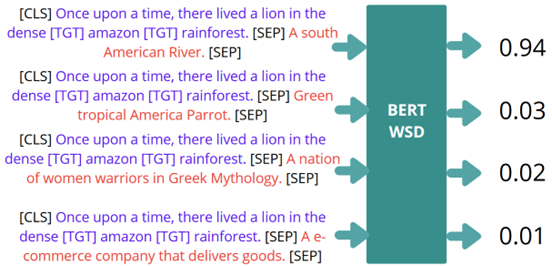
\includegraphics[scale=0.6]{img/bert_wsd.png}
    \caption{Het BERT WSD model}
\end{figure}

Naast foutieve antwoorden moet ook de vraag gegenereerd kunnen worden. Er wordt hiervoor gebruikt gemaakt van een getraind T5 Transformer model dat als invoer een blok tekst krijgt waarover er een vraag gesteld wordt en het antwoord op die vraag. Bv. \emph{“De rivier ontspringt in Peru en heeft een totale lengte van ongeveer 6.530 km. De Amazon is de tweede grootste rivier ter wereld”} en als antwoord willen we Amazon. Daarmee kan het na het trainen een vraag gaan genereren.

\subsubsection{Waar/onwaar-vraag}
\label{sec:waar/onwaar-vraag}
Bij een waar/onwaar-vraag wordt een uitspraak gegeven waarbij er Waar of Onwaar op geantwoord moet worden.
Vragen die waar zijn kunnen via abstractive of extractive summarization opgehaald worden. 
Het genereren van een onwaar-vraag kan op verschillende manieren:
\begin{itemize}
    \item Veranderen van benoemde entiteit (bv. Caesar naar Nero)
    \item Het toevoegen of verwijderen van een negatie  (bv. Het verandert ... naar Het verandert niet ... )
    \item Veranderen van bijvoeglijk naamwoord (bv. grootste naar kleinste)
    \item Veranderen van werkwoord (bv. aantrekken naar wegduwen)
\end{itemize}

Hiervoor kan Wordnet weer gebruikt worden om vragen die onwaar zijn te genereren.

\subsubsection{Invulvraag}
\label{sec:invulvraag}
Een invulvraag bestaat uit een zin waarbij een woord is weggelaten en is het de bedoeling om het juiste woord hier in te vullen.
Eerst worden de sleutelwoorden afgeleid uit de tekst. Dit proces wordt gedaan via de Python Keyword Extraction Library. Vanuit deze library zijn er keuzes om supervised of unsupervised modellen te gebruiken.\autocite{AIEngineering2021}

Supervised learning is een type machine learning-algoritme waarbij het model is getraind op gelabelde data, wat betekent dat de juiste uitvoer voor elk voorbeeld in de trainingdata is gegeven. Dit stelt het model in staat om voorspellingen te doen op nieuwe, ongeziene data op basis van de patronen die het heeft geleerd uit de trainingdata. In tegenstelling tot supervised learning is unsupervised learning een type machine learning-algoritme waarbij het model is getraind op ongelabelde data, wat betekent dat er geen juiste uitvoer is gegeven voor elk voorbeeld in de trainingdata. Het model moet de onderliggende structuur van de data zelf ontdekken.

Een reden om een unsupervised model te gebruiken is wanneer er geen gelabelde data beschikbaar is of wanneer het te kostbaar is om deze te verkrijgen. In deze gevallen kan unsupervised learning worden gebruikt om patronen en structuur in de data te vinden zonder dat er gelabelde voorbeelden nodig zijn. Een andere reden om unsupervised learning te gebruiken is om het aantal gelabelde data dat nodig is voor het trainen van een supervised model te verminderen. Door unsupervised learning te gebruiken voor preprocessing van de data, kan het mogelijk zijn om een nauwkeuriger en efficiënter supervised model te trainen op een kleinere dataset. Er wordt gebruikt gemaakt van een unsupervised model omdat er geen gelabelde data beschikbaar is in dit geval.

\subsubsection{Combinatievraag}
\label{sec:combinatievraag}
Bij een combinatievraag krijg je een aantal woorden en een aantal definities waarbij je ze juist moet verbinden. Voor het genereren volgt het bijna hetzelfde principe als een invulvraag. Er wordt weer gebruikt gemaakt van het Python Keyword Extraction Library om de keywords te bepalen. Een probleem hierbij is dat sommige keywords verschillende betekenissen kunnen hebben. Zoals bijvoorbeeld: Mouse kan een computermuis zijn of een dier. Dit probleem is hetzelfde als toen de meerkeuzevragen besproken en opgelost werden via het BERT WSD model als de volledige context wordt meegegeven. 

\subsection{Gamification}
\label{sec:gamification}

In en studie over de impact van gamificatie op studenten over gamificatie worden verschillende methodes besproken om gamificatie toe te passen in een educatieve omgeving. Een van de meest populaire methodes is het gebruik van een live leaderboard of top 10 scorebord. Dit kan bijvoorbeeld toegepast worden in een automatische quiz generator door de scores van gebruikers te vergelijken en ze te laten zien op een leaderboard, waardoor gebruikers gemotiveerd worden om hun prestaties te verbeteren en hoger te komen op het leaderboard. Badges, punten en rapporten om gebruikers te belonen voor het behalen van bepaalde doelen of het voltooien van specifieke taken geeft ook een positief resultaat in de betrokkenheid van de studenten. Dit kan bijvoorbeeld toegepast worden in een automatische quiz generator door gebruikers punten te geven voor het juist beantwoorden van vragen en badges te geven voor het behalen van hoge scores en op het einde van een quiz een rapport te tonen voor de gebruiker.\autocite{Smiderle2020}

Samengevat is er een verscheidenheid aan methodes die gebruikt kunnen worden in gamificatie voor een automatische quiz generator, zoals het gebruik van badges en punten, leaderboards en competitie en gegenereerde reports. Het is belangrijk om te kiezen welke methodes het best passen bij het doel van de quiz en de gebruikers om zo de meest effectieve gamificatie toe te passen.

% Hier beschrijf je de \emph{state-of-the-art} rondom je gekozen onderzoeksdomein, d.w.z.\ een inleidende, doorlopende tekst over het onderzoeksdomein van je bachelorproef. Je steunt daarbij heel sterk op de professionele \emph{vakliteratuur}, en niet zozeer op populariserende teksten voor een breed publiek. Wat is de huidige stand van zaken in dit domein, en wat zijn nog eventuele open vragen (die misschien de aanleiding waren tot je onderzoeksvraag!)?

% Je mag de titel van deze sectie ook aanpassen (literatuurstudie, stand van zaken, enz.). Zijn er al gelijkaardige onderzoeken gevoerd? Wat concluderen ze? Wat is het verschil met jouw onderzoek?

% Verwijs bij elke introductie van een term of bewering over het domein naar de vakliteratuur, bijvoorbeeld~\autocite{Hykes2013}! Denk zeker goed na welke werken je refereert en waarom.

% Draag zorg voor correcte literatuurverwijzingen! Een bronvermelding hoort thuis \emph{binnen} de zin waar je je op die bron baseert, dus niet er buiten! Maak meteen een verwijzing als je gebruik maakt van een bron. Doe dit dus \emph{niet} aan het einde van een lange paragraaf. Baseer nooit teveel aansluitende tekst op eenzelfde bron.

% Als je informatie over bronnen verzamelt in JabRef, zorg er dan voor dat alle nodige info aanwezig is om de bron terug te vinden (zoals uitvoerig besproken in de lessen Research Methods).

% Voor literatuurverwijzingen zijn er twee belangrijke commando's:
% \autocite{KEY} => (Auteur, jaartal) Gebruik dit als de naam van de auteur
%   geen onderdeel is van de zin.
% \textcite{KEY} => Auteur (jaartal)  Gebruik dit als de auteursnaam wel een
%   functie heeft in de zin (bv. ``Uit onderzoek door Doll & Hill (1954) bleek
%   ...'')

% Je mag deze sectie nog verder onderverdelen in subsecties als dit de structuur van de tekst kan verduidelijken.

%---------- Methodologie ------------------------------------------------------
\section{Methodologie}%
\label{sec:methodologie}
Er zal een PoC gebouwd worden in de vorm van een quiz generator die de Guidance Framework kan gebruiken om vragen te genereren. Hierbij zal eerst de data in via webscraping opgehaald worden van de Guidance Framework. De PoC wordt voorgesteld via een website gemaakt met Django. Het PoC kan 4 soorten vragen (meerkeuzevragen, waar/onwaar-vragen, ...) genereren en er wordt getest of de gegenereerde vragen accuraat genoeg zijn. 

Het testen van Natural Language Generation systemen is altijd een moeilijke taak geweest. Er wordt vooral gebruikt gemaakt van n-gram based similarity metrics (zoals bv. BLUE, NIST, ...) tegenwoordig wat enkel test hoeveel van een tekst voorkomt in een andere tekst. De BLUE score bleek wel een hogere score te krijgen dan de andere metrics maar er wordt nog altijd aangeraden om niet volledig hierop te steunen.\autocite{Nema2018} Er zal dus gebruikt worden gemaakt van niet alleen de BLUE score maar ook van de manuele score van een medewerker die het Guidance Framework kent. De medewerker zal een score geven van 1 tot 10 op relevantie. Dit wordt gedaan door een dataset van vragen te generen door de PoC. De grammatica van de gegenereerde vragen en antwoorden zullen ook getest worden. Dit gebeurt met part-of-speech tagging wat een proces is waarbij elk woord in een zin geclassificeerd wordt naar zijn syntactische functie, zoals een werkwoord, naamwoord, bijvoeglijk naamwoord, etc. Dit kan gebruikt worden om de grammatica van de zin te analyseren en te verifiëren of deze correct is.


% Hier beschrijf je hoe je van plan bent het onderzoek te voeren. Welke onderzoekstechniek ga je toepassen om elk van je onderzoeksvragen te beantwoorden? Gebruik je hiervoor literatuurstudie, interviews met belanghebbenden (bv.~voor requirements-analyse), experimenten, simulaties, vergelijkende studie, risico-analyse, PoC, \ldots?

% Valt je onderwerp onder één van de typische soorten bachelorproeven die besproken zijn in de lessen Research Methods (bv.\ vergelijkende studie of risico-analyse)? Zorg er dan ook voor dat we duidelijk de verschillende stappen terug vinden die we verwachten in dit soort onderzoek!

% Vermijd onderzoekstechnieken die geen objectieve, meetbare resultaten kunnen opleveren. Enquêtes, bijvoorbeeld, zijn voor een bachelorproef informatica meestal \textbf{niet geschikt}. De antwoorden zijn eerder meningen dan feiten en in de praktijk blijkt het ook bijzonder moeilijk om voldoende respondenten te vinden. Studenten die een enquête willen voeren, hebben meestal ook geen goede definitie van de populatie, waardoor ook niet kan aangetoond worden dat eventuele resultaten representatief zijn.

% Uit dit onderdeel moet duidelijk naar voor komen dat je bachelorproef ook technisch voldoen\-de diepgang zal bevatten. Het zou niet kloppen als een bachelorproef informatica ook door bv.\ een student marketing zou kunnen uitgevoerd worden.

% Je beschrijft ook al welke tools (hardware, software, diensten, \ldots) je denkt hiervoor te gebruiken of te ontwikkelen.

% Probeer ook een tijdschatting te maken. Hoe lang zal je met elke fase van je onderzoek bezig zijn en wat zijn de concrete \emph{deliverables} in elke fase?

%---------- Verwachte resultaten ----------------------------------------------
\section{Verwacht resultaat, conclusie}%
\label{sec:verwachte_resultaten}
Uit dit onderzoek moet blijken of een quiz generator geschikt is om vragen te genereren uit het Info Support Guidance Framework. De PoC zal een goeie indicator zijn hiervoor met een hoge BLUE score en een hoge manuele score van een medewerker van Info Support. Echter doordat er het Guidance Framework wordt gewebscraped zal een gelijkaardige structuur moeten behouden worden en in het Engels blijven geschreven worden indien er ze het Guidance Framework uitbreiden om de PoC te kunnen blijven gebruiken. Hopelijk zal de PoC kunnen gebruikt worden door Info Support om te helpen hun kennis van het Guidance Framework op te frissen.

% Hier beschrijf je welke resultaten je verwacht. Als je metingen en simulaties uitvoert, kan je hier al mock-ups maken van de grafieken samen met de verwachte conclusies. Benoem zeker al je assen en de onderdelen van de grafiek die je gaat gebruiken. Dit zorgt ervoor dat je concreet weet welk soort data je moet verzamelen en hoe je die moet meten.

% Wat heeft de doelgroep van je onderzoek aan het resultaat? Op welke manier zorgt jouw bachelorproef voor een meerwaarde?

% Hier beschrijf je wat je verwacht uit je onderzoek, met de motivatie waarom. Het is \textbf{niet} erg indien uit je onderzoek andere resultaten en conclusies vloeien dan dat je hier beschrijft: het is dan juist interessant om te onderzoeken waarom jouw hypothesen niet overeenkomen met de resultaten.



\printbibliography[heading=bibintoc]
    
\end{document}